\documentclass[12pt]{article}
\usepackage[margin=1.25in]{geometry}
\usepackage{fontenc}
\usepackage{babel}
\usepackage{float}
\usepackage{graphicx} % images
\usepackage{fancyhdr} % header and footer
\usepackage{algorithm}
\usepackage{algorithmic}
\usepackage{nameref}
\makeatletter
\newcommand*{\currentname}{\@currentlabelname}
\makeatother

% Page Styling
\pagestyle{fancy}
\lhead{MSE 310 Course Project}
\rhead{\thepage}
\lfoot{Simon Fraser University}
\cfoot{}

\title{
  ICT3 Industrial Control Graphical User Interface
}
\author{
  Bansal, Neeraj\\
  \texttt{301xxxxx}
  \and
  Eshikena, Elvis\\
  \texttt{30132117}
}

\begin{document}
\maketitle

% %%%%%%%%%%%%%%%%%%%%%%%%%%%%%%%%%%%
% Abstract
% %%%%%%%%%%%%%%%%%%%%%%%%%%%%%%%%%%%
\begin{abstract}
  The use of automation technology in the world is wide\-spread and a growing field.
  Automation is used every\-where from software tasks to machine tasks. The ICT3 platform
  is a typical representation of an industrial automation setup. The objective of this
  project is to use LabVIEW to develop an efficient and robust, fully automated 
  controller for the ICT3 setup to asssemble widgets.
  \bigbreak
  The method used for the base controller was an event prog\-ramming struc\-ture. The
  Graphical User Interface GUI was designed for ease of use and learn-time. At
  every clock-cycle, all the sensors where scanned for data. When the rigth
  sequence of data was read, the corresponding actuator action and program data
  were executed and updated respectively.
  \bigbreak
  The results of the system showed that ...\% of efficiency from a time run of ..
  and .. was also present in the system.
  \bigbreak
  The project demostrated how LabVIEW can be used to program a complex controller
  to automate the ICT3 platform and generate its runtime results
\end{abstract}
\newpage

\tableofcontents
\newpage

% %%%%%%%%%%%%%%%%%%%%%%%%%%%%%%%%%%%
% Introductions
% %%%%%%%%%%%%%%%%%%%%%%%%%%%%%%%%%%%
\section{Introduction}
  The ICT3 platform is a representation of a typical industrial automation 
  system. The system includes component sorting, assembly inspection and 
  accepts/reject processes. When connected through an interface card or a 
  Programmable Logic Controller, the system can
  be controlled through a PC.
  \bigbreak
  Using a PC, the sensors and actuators can be programmed to
  take-in data through the sensors and manipulate the workspace using the 
  actauators.
  \bigbreak
  The objective of the project is to develop an efficient and robust, fully 
  automated controller for the ICT setup to asssemble widgets.

% %%%%%%%%%%%%%%%%%%%%%%%%%%%%%%%%%%%
% System Overview
% %%%%%%%%%%%%%%%%%%%%%%%%%%%%%%%%%%%
\section{System Overview}
  \subsection{System Function}
    \subsubsection{System Cycle}
      The system is designed to sort between a metal peg and a plastic ring, assemble
      the plastic ring on the metal peg and then determine if the assembly was done 
      correctly. It then discards or accepts the item based on the assembly status.

    \subsubsection{Sorting Area}
      % \begin{figure}[h!]
      %   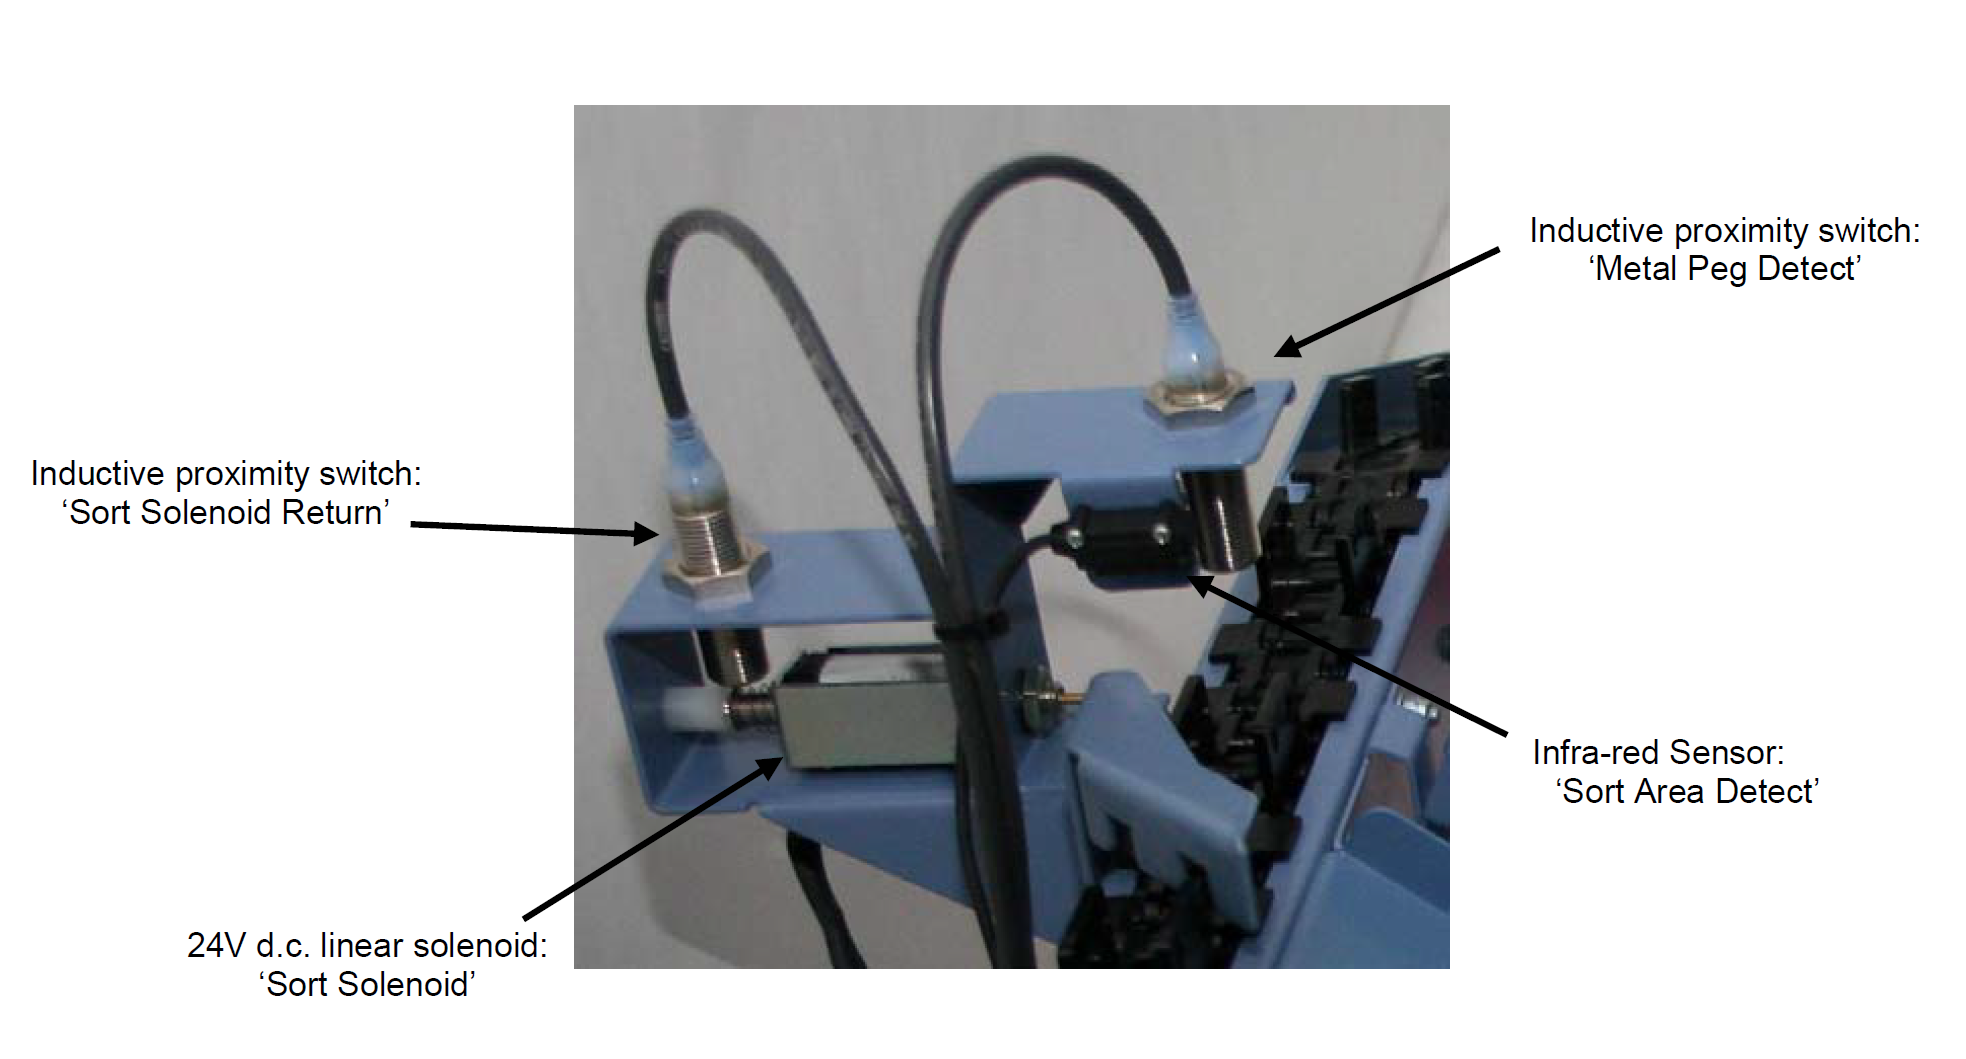
\includegraphics[width=\linewidth]{images/sorting-area.png}
      %   \caption{ICT3 Sorting Area}
      %   \label{fig:sorta}
      % \end{figure}

      At the sorting area, the chain conveyor brings the metal pegs will be sep\-erated
      from the plastic rings. The part will be detected by the $Sort\-Area\-Detector$ 
      sensor. The sensor is position where the part will also be infront of the 
      $SortSolenoid$. If the part is a ring, the solenoid hits it into the 
      assembly chute, if not, it allows it pass down a feeder chute onto the belt
      conveyor.

    \subsubsection{The Assembly Area}
      When the ring enters the assembly chute, it is staged in the $RingQueue$
      by the $RotarySolenoid$. When the $RingQueue$ holds 5 rings, further rings are
      allowed to pass the sorting area.
      \bigbreak
      When the $AssemblyHopperFull$ sensor detects that the hopper is empty, the 
      $RotarySolenoid$ allows a ring to be dispensed from the $RingQueue$ into the
      into the hopper and also decrements the $RingQueue$.
      \bigbreak
      When the peg reaches the hopper, it is directed to engage with the hole in the ring
      which makes a complete widget assembly.

    \subsubsection{The Sensing Station}
      At the sensing station, the sesnsors detect if a com\-ponent was ass\-embled or if the
      com\-ponent is a peg or ring. There are three sensors available $Belt\-Peg\-Detect$, 
      $Sensing\-Area\-Detect$ and the $Ring\-Assembled$. The output from this area is the type
      of component which is passing the switch.
      \begin{itemize}
        \item Plastic Ring
        \item Metal Peg
        \item Assembled Ring and Peg
      \end{itemize}

    \subsubsection{The Reject Station}
      When the component from the sensing station is detected by the $Reject\-Area\-Detect$
      sensor, it uses the data from the sensing station to act on the component. If it
      is either a single ring or peg, the $RejectSolenoid$ is activated. It allows an
      assembled part to pass through.

  \subsection{GUI Design}
  \subsection{Program Design}
    % %%%%%%%%%%%%%%%%%%%%%%%%%%%%%%%%%%%
% Algorithms
% %%%%%%%%%%%%%%%%%%%%%%%%%%%%%%%%%%%
\section{Algorithms}
  This section highlights the logic if the different sections of the system.
  Here is a list of program variables which will be tracked and referenced
  \begin{itemize}
    \item $PegCount$
    \item $RingCount$
    \item $RingQueue$
    \item $AssembledCount$
    \item $RejectedPegCount$
    \item $RejectedRingCount$
  \end{itemize}

  \subsection{The Sorting Area}
    \begin{algorithm}[H]
      \caption{\currentname}
      \begin{algorithmic}
        \REQUIRE $t$ - time count
        \REQUIRE {
          $SortAreaDetect$, $Sort\-Metal\-Detect$, $Sort\-Solenoid\-Return$ are the sensor data
        }
        \REQUIRE $SortSolenoid$ an output reference to the actuator
        \STATE $A \Leftarrow SortAreaDetect$
        \STATE $M \Leftarrow MetalPegDetect$
        \STATE $S \Leftarrow SortSolenoidReturn$
        \WHILE {$ProgramIsRunning$}
          \IF{$[t]=1\,and\,A[t-1]=0$}
            \IF{$M[t]=M[t-1]$}
            \STATE $SortSolenoid \leftarrow 1$
            \STATE $RingCount \leftarrow RingCount + 1$
            \ELSE
              \STATE $PegCount \leftarrow PegCount + 1$
            \ENDIF
          \ENDIF

          \IF{$S[t]=1 \land S[t-1]=0$}
            \STATE $RingQueue \leftarrow RingQueue + 1$
          \ENDIF
        \ENDWHILE
      \end{algorithmic}
    \end{algorithm}

  \subsection{The Assembly Area}
    \begin{algorithm}[H]
      \caption{\currentname}
      \begin{algorithmic}
        \REQUIRE $t$, The time count
        \REQUIRE $SortSolenoid$
        \REQUIRE $RingQueue$
        \REQUIRE $RotarySolenoid$
        \REQUIRE $HopperFull$
        \WHILE {$ProgramIsRunning$}
          \IF {$HopperIsEmpty \land (RingQueue \geq 2)$} 
            \STATE $RotarySolenoid \leftarrow 1$
            \STATE $RingQueue \leftarrow RingQueue - 1$
          \ELSIF {$HopperIsEmpty \land PegDetected \land (RingQueue \geq 1)$ }
            \STATE $RotarySolenoid \leftarrow 1$
            \STATE $RingQueue \leftarrow RingQueue - 1$
          \ELSE
            \STATE $RotarySolenoid \leftarrow 0$
          \ENDIF
        \ENDWHILE
      \end{algorithmic}
    \end{algorithm}

  \subsection{The Sensing Station}
    \begin{algorithm}[H]
      \caption{\currentname}
      \begin{algorithmic}
        \REQUIRE $t$, The time count
        \REQUIRE $PEG$ Flag
        \REQUIRE $ASSEMBLED$ Flag
        \REQUIRE $SensingAreaDetect$
        \REQUIRE $BeltPegDetect$
        \REQUIRE $RingAssembledDetect$
        \STATE $A \Leftarrow SensingAreaDetect$
        \STATE $P \Leftarrow BeltPegDetect$
        \WHILE {$ProgramIsRunning$}
          \IF {$RingAssembledDetect$}
            \STATE $ASSEMBLED \leftarrow 1$
          \ENDIF

          \IF {$BeltPegDetect$}
            \STATE $PEG \leftarrow 1$
          \ENDIF

          \IF {$A[t]=1 \land A[t-1]=0$}
            \IF {$ASSEMBLED=1$}
              \STATE $RejectionControl \leftarrow 1$
              \STATE $ASSEMBLED \leftarrow 0$
            \ELSE [ASSEMBLED Flag not set]
              \IF {$PEG=1$}
                \STATE $RejectionControl \leftarrow 2$
                \STATE $PEG \leftarrow 0$
              \ELSE [PEG flag not set]
                \STATE $RejectionControl \leftarrow 3$              
              \ENDIF
            \ENDIF
          \ENDIF
        \ENDWHILE        
      \end{algorithmic}
    \end{algorithm}

  \subsection{The Reject Area}
    \begin{algorithm}[H]
      \caption{\currentname}
      \begin{algorithmic}
        \REQUIRE $t$, The time count
        \REQUIRE $RejectionControl$
        \REQUIRE $PEG$ Flag
        \REQUIRE $ASSEMBLED$ Flag
        \REQUIRE $RejectAreaDetect$
        \REQUIRE $RejectSolenoid$
        \REQUIRE $RejectSolenoidReturn$
        \REQUIRE $AssembledCount$
        \REQUIRE $RejectedPegCount$
        \REQUIRE $RejectedRingCount$
        \STATE $A \Leftarrow RejectAreaDetect$
        \STATE $R \Leftarrow RejectSolenoidReturn$
        \WHILE {$ProgramIsRunning$}
          \IF {$A[t]=1 \land A[t-1]=0$}
            \IF {$RejectionControl=1$}
              \STATE $RejectSolenoid \leftarrow 0$
              \STATE $AssembledCount \leftarrow AssembledCount + 1$
            \ELSIF {$RejectionControl=2$}
              \STATE $RejectSolenoid \leftarrow 1$
              \STATE $RejectedPegCount \leftarrow RejectedPegCount + 1$
            \ELSIF {$RejectionControl=3$}
              \STATE $RejectSolenoid \leftarrow 1$
              \STATE $RejectedRingCount \leftarrow RejectedRingCount + 1$
            \ELSE [No predefined state]
              \STATE Do nothing
            \ENDIF
            \STATE $RejectionControl \leftarrow 0$
          \ENDIF
        \ENDWHILE
      \end{algorithmic}
    \end{algorithm}

% %%%%%%%%%%%%%%%%%%%%%%%%%%%%%%%%%%%
% Discussions
% %%%%%%%%%%%%%%%%%%%%%%%%%%%%%%%%%%%
\section{Summary}
  \subsection{Performace}
  \subsection{Reccomendations}
% %%%%%%%%%%%%%%%%%%%%%%%%%%%%%%%%%%%
% Conclusions
% %%%%%%%%%%%%%%%%%%%%%%%%%%%%%%%%%%%
\section{Conclusions}
  Concluding sentences

\end{document}
